%%%%%%%%%%%%%%%%%%%%%%%%%%%%%%%%%%%%%%%%%
% Stylish Article
% LaTeX Template
% Version 2.1 (1/10/15)
%
% This template has been downloaded from:
% http://www.LaTeXTemplates.com
%
% Original author:
% Mathias Legrand (legrand.mathias@gmail.com) 
% With extensive modifications by:
% Vel (vel@latextemplates.com)
% Final ACS by:
% Juan Barbosa
% License:
% CC BY-NC-SA 3.0 (http://creativecommons.org/licenses/by-nc-sa/3.0/)
%
%%%%%%%%%%%%%%%%%%%%%%%%%%%%%%%%%%%%%%%%%
\documentclass[fleqn,10pt]{SelfArx}
%\usepackage[superscript]{cite}
\usepackage{wrapfig}
%----------------------------------------------------------------------------------------
%	ARTICLE INFORMATION
%----------------------------------------------------------------------------------------

\JournalInfo{Laboratorio Org\'anica 3, No. 2, 25/08/2017} % Journal information
\Archive{ }

\PaperTitle{Reacci\'on de McMurry} %
%\Keywords{Keyword1 --- Keyword2 --- Keyword3} % Keywords - if you don't want any simply remove all the text between the curly brackets
%\newcommand{\keywordname}{Keywords} % Defines the keywords heading name

%----------------------------------------------------------------------------------------
%	ABSTRACT
%----------------------------------------------------------------------------------------

\Abstract{
\begin{wrapfigure}{r}{0.45\textwidth}
	\centering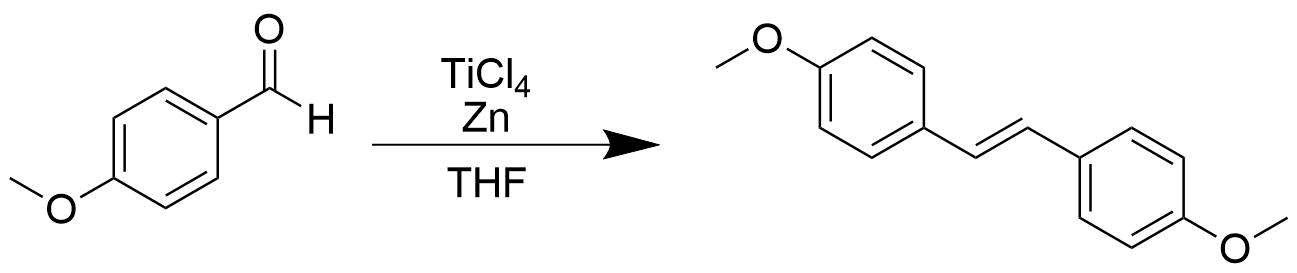
\includegraphics[width=0.9\linewidth]{structures/Reaction.png}
\end{wrapfigure}
}

%----------------------------------------------------------------------------------------

\begin{document}

\flushbottom % Makes all text pages the same height

\maketitle % Print the title and abstract box

%\tableofcontents % Print the contents section

\thispagestyle{empty} % Removes page numbering from the first page



%----------------------------------------------------------------------------------------
%	ARTICLE CONTENTS
%----------------------------------------------------------------------------------------

\section*{Introducci\'on} % The \section*{} command stops section numbering
%------------------------------------------------

\section{Resultados y Discusi\'on}
\begin{scheme}[h]
	\centering
	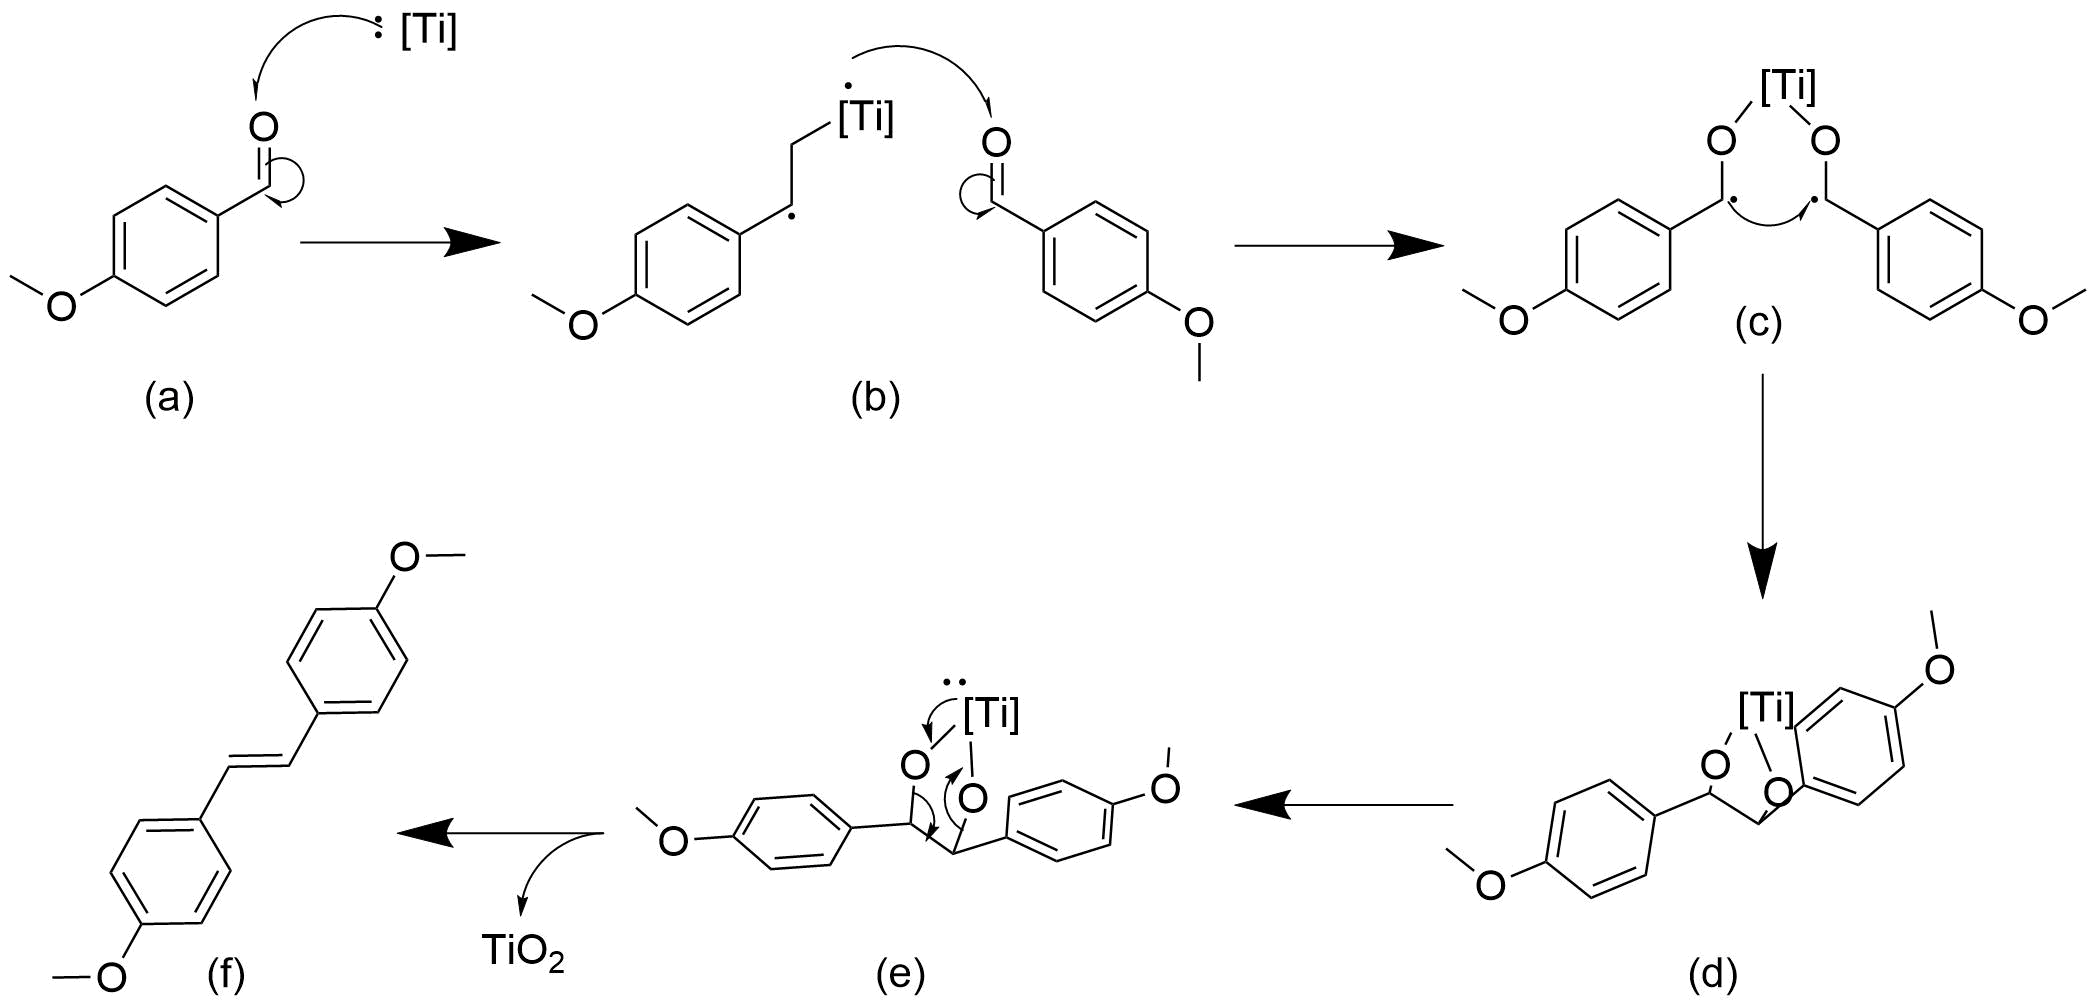
\includegraphics[width = \linewidth]{structures/mechanism.png}
	\caption{Mecanismo de reacci\'on propuesto.}
\end{scheme}

\section{Conclusiones}
\section{Secci\'on experimental}
50 mL de tetrahidrofurano previamente seco por 48 horas usando tamiz molecular, se agregan sobre un bal\'on de dos bocas junto con Zinc (15.0 mmol) y cloruro de titanio (7.5 mmol). La soluci\'on se lleva a reflujo por 1 hora, pasada la cual se adiciona \textit{p}-metoxibenzaldehido (5.0 mmol). La reacci\'on se lleva a cabo a 55 $^\circ$C por 18 horas. La reacci\'on es tratada en 50 mL de \'acido clorh\'idrico 1 M. Se realiza una filtraci\'on en celita y una extracci\'on l\'iquido l\'iquido con dos lavados de 15 mL de diclorometano. El extracto se baña en salmuera y se extrae el sobrenadante, el cual se seca usando sulfato de magnesio y se evapora el disolvente.
%----------------------------------------------------------------------------------------
%	REFERENCE LIST
%----------------------------------------------------------------------------------------
\phantomsection
\bibliography{informe}
\bibliographystyle{unsrt}

%----------------------------------------------------------------------------------------
\newpage
\onecolumn
\section{Informaci\'on suplementaria}\label{sec: complementaria}
\end{document}